\section{Hamiltonian comparison}\label{sec:cmp}

This section produces the comparison data of Definition~\ref{def:mech-datum}. Let $\Delta$ be a compact
full-dimensional downward polytope with outer faces $\langle b_\nu,p\rangle\le\ell_\nu$ (\S\ref{sec:mech-interfaces}),
let $V_\Delta=\{w\in\C^m:p(w)\in\Delta\}$ be its toric domain, with $p_j=\pi|w_j|^2$, $\theta_j=\arg w_j/2\pi\in\R/\Z$
and $\omega_V=\sum_jdp_j\wedge d\theta_j$ as in \S\ref{sec:mech}, and let $P$ be a continuous concave function on $\Delta$
with positive mean; in the general construction $P$ is rational concave piecewise affine and positive off a core
$\tau_\Delta\Delta$. We seek a smooth toric function $K$ and a Hamiltonian isotopy $q_t$ of $V_\Delta$ with
$(K-P)\circ p\circ q_1\le K\circ p-\gamma$ for some $\gamma>0$. Since $q_1$ preserves the measure $\omega_V^m/m!$ and,
the angles having period $1$, $p_*(\omega_V^m/m!)$ is Lebesgue measure on $\Delta$, the map $q_1$ can only redistribute
the values of $K-P$; the inequality asks that after redistribution they lie below $K-\gamma$. The construction has
two halves: a scalar half (rearrangement operators on convex functions on $\Delta$ and a contraction whose
approximate fixed point is $K$, \S\S\ref{sec:cmp-rearrangement}--\ref{sec:cmp-fixed}) and a symplectic half
(isotopies realising one coordinate rearrangement up to a prescribed error, \S\ref{sec:cmp-realisation}).

The rearrangement operator and the contraction are those of \cite[\S2]{OpenAI2026}. We replace the fixed point by a
finite rational iterate with explicit iteration count and gap (Proposition~\ref{prop:cmp-fixed-point}), and the
existence of realising isotopies by explicit Hamiltonians (Theorem~\ref{thm:cmp-realisation}). For $k\ge10$ equal
balls in dimension four with $\frac34<\rho\sqrt k<1$ no fixed point is needed: $K$ is linear, the rearranged inequality
is an identity, and the inner planar map costs at most $g/32$ of the gap (\S\ref{sec:cmp-linear}). Every object defined in this section is explicit at level L1
(Definition~\ref{def:intro-levels}).

The polyhedral iterate with log-sum-exp smoothing (Theorem~\ref{thm:cmp-main}) is used for all
higher-dimensional models. The general four-dimensional case uses the scalar version of \Ssec{sec:scalar-cmp}, in
which the finite iterate is extended by an infimal formula and smoothed by convolution with a fixed bump; its gap
and its planar Hamiltonian are \Sref{Proposition}{prop:scalar-cmp-gap} and
\Sref{Proposition}{prop:scalar-planar-realisation}. The four-dimensional equal-ball case with $k\ge10$ uses the linear
datum of \S\ref{sec:cmp-linear}.

Throughout, fibre Hamiltonians follow the convention $\iota_{X_Q}\omega_V=-dQ$ of
Definition~\ref{def:mech-datum}. Norms $\|\cdot\|$ are uniform norms on $\Delta$. For a coordinate $j$ we write
$p=(y,x)$ with $x=p_j$ and $y=(p_i)_{i\ne j}$. The polytope $\Delta$ is \emph{rational} if all $b_\nu,\ell_\nu$ are
rational. A function on $\Delta$ is \emph{rational convex polyhedral} if it is the restriction to $\Delta$ of
$\max_{\iota\in I}\phi_\iota$ for a finite family of affine functions $\phi_\iota$ with rational coefficients, and
\emph{rational concave piecewise affine} if it is $\min_{\iota\in I}\phi_\iota$ for such a family. All cutoffs and
clocks below use the flat step $S$ of \Sref{Definition}{def:pre-flat}, all of whose derivatives vanish at $0$ and
$1$.

\subsection{Coordinate rearrangement}\label{sec:cmp-rearrangement}

Fix $j$. Because every $b_\nu$ is nonnegative and $\Delta$ is compact, at least one $\nu$ has $b_{\nu j}>0$, and
\[
 L(y)=\min_{\nu:\,b_{\nu j}>0}\frac{\ell_\nu-\sum_{i\ne j}b_{\nu i}y_i}{b_{\nu j}}
\]
is a continuous concave piecewise affine function on the projection $\Delta_j=\{y:(y,0)\in\Delta\}$, with
$\Delta=\{(y,x):y\in\Delta_j,\ 0\le x\le L(y)\}$. The slice of $\Delta$ through $y$ is the interval $[0,L(y)]$.

\begin{definition}[Coordinate rearrangement]\label{def:cmp-rearrangement}
For a continuous convex function $F$ on $\Delta$ and a coordinate $j$, put
\[
 (R_jF)(y,x)=\min_{\substack{0\le a,\ a+x\le L(y)}}\ \max\bigl(F(y,a),\,F(y,a+x)\bigr),
 \qquad (y,x)\in\Delta,
\]
and $\Rcal=R_m\circ\dots\circ R_1$.
\end{definition}

The minimum exists because the admissible $a$ form the compact interval $[0,L(y)-x]$. Since the sublevel sets of
a convex function of one variable are intervals, $x\mapsto(R_jF)(y,x)$ is the increasing rearrangement of
$F(y,\cdot)$ on $[0,L(y)]$ with respect to Lebesgue measure: for $x>0$ it is the smallest value $b$ for which
$\{F(y,\cdot)\le b\}$ has length at least $x$; at $x=0$ it equals $\min F(y,\cdot)$.

\begin{lemma}[Properties of $R_j$]\label{lem:cmp-rearrangement}
\uses{def:cmp-rearrangement, S-lem:fcp-rearrangement, S-lem:fcp-polyhedral}
Let $F,G$ be continuous convex functions on $\Delta$ and $j\in\{1,\dots,m\}$.
\begin{enumerate}[label=(\roman*)]
\item $R_jF$ is continuous and convex on $\Delta$, and $\int_\Delta R_jF=\int_\Delta F$.
\item If $F\le G$ then $R_jF\le R_jG$; $R_j(F+c)=R_jF+c$ and $R_j(\alpha F)=\alpha R_jF$ for constants $c\in\R$,
 $\alpha\ge0$; $\|R_jF-R_jG\|\le\|F-G\|$.
\item For each $y$, $x\mapsto(R_jF)(y,x)$ is nondecreasing, $(R_jF)(y,0)=\min_{[0,L(y)]}F(y,\cdot)$ and
 $(R_jF)(y,L(y))=\max_{[0,L(y)]}F(y,\cdot)$; in particular $\max_\Delta R_jF=\max_\Delta F$.
\item If $F$ is nondecreasing in $p_i$ for some $i\ne j$, so is $R_jF$. Consequently $\Rcal F$ is
 nondecreasing in every coordinate, and $\Rcal F(0)=\min_\Delta\Rcal F$.
\item Let $\Delta$ be rational. If $F$ is rational convex polyhedral, so is $R_jF$. If $F=\max_{\iota\in I}\phi_\iota$,
 the epigraph of $R_jF$ over $\Delta$ is the projection to $(y,x,t)$ of the rational polyhedron in the variables
 $(y,x,t,a)$ defined by $p=(y,x)\in\Delta$, $a\ge0$, $b_{\nu j}(a+x)+\sum_{i\ne j}b_{\nu i}y_i\le\ell_\nu$ for every
 $\nu$ with $b_{\nu j}>0$, and $t\ge\phi_\iota(y,a)$, $t\ge\phi_\iota(y,a+x)$ for every $\iota\in I$; eliminating $a$
 by Fourier--Motzkin elimination gives finitely many rational affine functions whose maximum is $R_jF$.
\end{enumerate}
\end{lemma}

\begin{proof}
The proofs are in \Sref{Lemma}{lem:fcp-rearrangement} and \Sref{Lemma}{lem:fcp-polyhedral}; we give the arguments
for convexity, monotonicity and (v). Convexity: if $[a_0,a_0+x_0]$ and $[a_1,a_1+x_1]$ are minimising intervals on
the slices through $y_0$ and $y_1$, their convex combination with weights $1-\vartheta,\vartheta$ is admissible on the
slice through $(1-\vartheta)y_0+\vartheta y_1$ (concavity of $L$), and convexity of $F$ bounds its endpoint values by
the corresponding convex combinations. Monotonicity in $p_i$: lowering $y_i$ does not shrink the slice, because
$b_{\nu i}\ge0$, so every admissible interval stays admissible while its endpoint values do not increase. Item (v):
the minimum in Definition~\ref{def:cmp-rearrangement} is attained, so $t\ge R_jF(y,x)$ if and only if some $a$
satisfies the displayed system, and the epigraph is the projection. The variable $t$ occurs only in lower bounds
$t\ge\dots$, and Fourier--Motzkin elimination of $a$ forms nonnegative combinations of the given inequalities; so it
produces only inequalities of the form $t\ge$ (affine function of $(y,x)$) and inequalities free of $t$. The latter
hold on $\Delta$, because every $(y,x)\in\Delta$ has a feasible $a$ (for instance $a=0$, with $t$ large), and hence
$R_jF$ is the maximum of the former.
\end{proof}

\subsection{A finite comparator iteration}\label{sec:cmp-fixed}

For $0<\lambda<1$ consider $T_\lambda(F)=\Rcal(\lambda F-P)$ on the space of continuous convex functions on $\Delta$.
If $P$ is concave, $\lambda F-P$ is convex, and by Lemma~\ref{lem:cmp-rearrangement}(ii) $T_\lambda$ is a
contraction with constant $\lambda$.

\begin{proposition}[Finite comparator]\label{prop:cmp-fixed-point}
\uses{lem:cmp-rearrangement, S-prop:fcp-fixed-point}
Let $\Delta$ be rational, $\tau_\Delta\in(0,1)$ rational, and $P$ a rational concave piecewise affine function on
$\Delta$ with mean $\mu=\vol(\Delta)^{-1}\int_\Delta P>0$ and $P\ge\beta_P$ on $\Delta\setminus\tau_\Delta\Delta$ for some
$\beta_P>0$. Let $d$ be rational with $0<d<\min(\mu,\beta_P)$ and put
\[
 \eta_\Delta=(1-\tau_\Delta)(\mu-d),\qquad M_P=\max\bigl(1,\ d-\min_\Delta P+1\bigr),\qquad
 \lambda=1-\frac{\eta_\Delta}{2(M_P+\eta_\Delta)}.
\]
Define $K_0=0$, $K_{r+1}=\Rcal(\lambda K_r-P)$ and
\[
 N=\left\lceil\frac{16\|P\|}{d(1-\lambda)(\lambda^{-1}-1)}\right\rceil+1.
\]
Then every $K_r$ is rational convex polyhedral, $\lambda^N\|P\|/(1-\lambda)<d/16$, and
\[
 \Rcal(K_N-P)\le K_N-\tfrac78d\qquad\text{on }\Delta .
\]
\end{proposition}

All quantities in Proposition~\ref{prop:cmp-fixed-point} are computed by finite rational arithmetic. For a
rational convex polyhedral $G$, Lemma~\ref{lem:cmp-rearrangement}(iii),(iv) give $\min_\Delta G=(\Rcal G)(0)$, and
the maximum of an affine function $\phi$ is $-\min_\Delta(-\phi)$; this gives $\min_\Delta P$ and $\|P\|$ by
Fourier--Motzkin elimination. The integral $\int_\Delta P$, hence $\mu$, is computed by iterated integration of
rational polynomials over rational polyhedral cells, one coordinate at a time
(\Sref{Proposition}{prop:fcp-fixed-point}(a)). Hence $N$ is obtained by rational arithmetic and a ceiling, and
$K_N$ by $mN$ Fourier--Motzkin eliminations (Lemma~\ref{lem:cmp-rearrangement}(v)).

\begin{proof}
\emph{Rationality.} $K_0=0$, and if $K_r=\max_\iota\phi_\iota$ and $P=\min_u\psi_u$ with rational affine
$\phi_\iota,\psi_u$, then $\lambda K_r-P=\max_{\iota,u}(\lambda\phi_\iota-\psi_u)$ is rational convex polyhedral, so
$K_{r+1}$ is by Lemma~\ref{lem:cmp-rearrangement}(v) applied $m$ times.

\emph{The fixed point.} The continuous convex functions on $\Delta$ form a closed subset of $C(\Delta)$, so the
$\lambda$-contraction $T_\lambda$ has a unique fixed point $K_\lambda$ (the comparison function of
\cite[\S2.2]{OpenAI2026}), and $\|K_r-K_\lambda\|\le\lambda^r\|K_\lambda\|$. Since $\Rcal0=0$ and $\Rcal$ is
$1$-Lipschitz, $\|K_\lambda\|\le\lambda\|K_\lambda\|+\|P\|$, so $\|K_\lambda\|\le\|P\|/(1-\lambda)$. By
Lemma~\ref{lem:cmp-rearrangement}(i),(iv), $K_\lambda$ is convex, nondecreasing in every coordinate,
$K_\lambda(0)=\min K_\lambda$, and integrating the fixed-point equation gives
$\int K_\lambda=\lambda\int K_\lambda-\int P$, that is, the mean of $K_\lambda$ is $-\mu/(1-\lambda)$.

\emph{The gap of the fixed point.} Note $\tfrac12<\lambda<1$, $1-\lambda=\eta_\Delta/(2(M_P+\eta_\Delta))$ and
\begin{equation}\label{eq:cmp-lambda}
 \frac{\lambda\eta_\Delta}{1-\lambda}=2M_P+\eta_\Delta>d-\min_\Delta P .
\end{equation}
The idea is that the mean of $K_\lambda$ is very negative, so by convexity its values on the core
$\tau_\Delta\Delta$ lie well below its maximum, while off the core $P\ge\beta_P$ lowers $\lambda K_\lambda-P$; the
fixed-point equation then forces the maximum of $K_\lambda$ to be negative. In detail, let $M_\lambda=\max K_\lambda$ and suppose $M_\lambda\ge-d/(1-\lambda)$, so that
$\lambda M_\lambda\le M_\lambda+d$. If $p\in\Delta\setminus\tau_\Delta\Delta$, then
$\lambda K_\lambda(p)-P(p)\le\lambda M_\lambda-\beta_P<M_\lambda$, because $(1-\lambda)M_\lambda\ge-d>-\beta_P$. If
$p=\tau_\Delta v$ with $v\in\Delta$, convexity and $K_\lambda(0)=\min K_\lambda\le-\mu/(1-\lambda)$ give
\[
 K_\lambda(p)\le\tau_\Delta M_\lambda+(1-\tau_\Delta)K_\lambda(0)
 \le M_\lambda-(1-\tau_\Delta)\Bigl(M_\lambda+\frac{\mu}{1-\lambda}\Bigr)\le M_\lambda-\frac{\eta_\Delta}{1-\lambda},
\]
the last step by $M_\lambda\ge-d/(1-\lambda)$. Hence, by \eqref{eq:cmp-lambda},
\[
 \lambda K_\lambda(p)-P(p)\le M_\lambda+d-\frac{\lambda\eta_\Delta}{1-\lambda}-\min_\Delta P<M_\lambda .
\]
Thus $\max_\Delta(\lambda K_\lambda-P)<M_\lambda$, while Lemma~\ref{lem:cmp-rearrangement}(iii) and the fixed-point
equation give $M_\lambda=\max\Rcal(\lambda K_\lambda-P)=\max(\lambda K_\lambda-P)$, a contradiction. Therefore
$M_\lambda<-d/(1-\lambda)$, i.e.\ $(1-\lambda)K_\lambda<-d$ on $\Delta$, and by Lemma~\ref{lem:cmp-rearrangement}(ii)
\[
 \Rcal(K_\lambda-P)=\Rcal\bigl(\lambda K_\lambda-P+(1-\lambda)K_\lambda\bigr)\le\Rcal(\lambda K_\lambda-P)-d=K_\lambda-d .
\]

\emph{The finite iterate.} Let $r_N=\|K_N-K_\lambda\|\le\lambda^N\|P\|/(1-\lambda)<d/16$. By
Lemma~\ref{lem:cmp-rearrangement}(ii),
$\Rcal(K_N-P)\le\Rcal(K_\lambda-P)+r_N\le K_\lambda-d+r_N\le K_N-d+2r_N<K_N-\tfrac78d$.
\end{proof}

The construction applies verbatim when the polytope and the affine pieces have real coefficients:
Fourier--Motzkin elimination uses finitely many arithmetic operations and comparisons, and the estimates are
unchanged, with ``rational convex polyhedral'' replaced by ``convex polyhedral''. The same holds for the smoothing
and realisation statements below. This real version is the one used for real capacities.

\subsection{Realisation and the comparison datum}\label{sec:cmp-realisation}

The symplectic half realises one coordinate rearrangement by an isotopy which changes only the $j$-th
moment; the other fibre coordinates may rotate.

\begin{theorem}[Realisation of one coordinate rearrangement]\label{thm:cmp-realisation}
\lean[needed]{SymplecticPacking.HighDim.liftGen_spec}
\uses{lem:cmp-rearrangement, S-def:plc-slice, S-thm:plc-lift, S-thm:pln-isotopy}
Let $\Delta$ be rational, $F$ rational convex polyhedral on $\Delta$, $j\in\{1,\dots,m\}$ and $e>0$ rational. Let
$Q^{(j)}_t$ be the Hamiltonian defined from $(\Delta,F,j,e)$ in \Sref{Definition}{def:plc-slice}, and let
$(q^{(j)}_t)_{t\in[0,1]}$ be its flow ($\iota_{X}\omega_V=-dQ^{(j)}_t$). Then $Q^{(j)}$ is smooth with compact support
in $w$, $(q^{(j)}_t)$ is a smooth Hamiltonian isotopy of $\C^m$, and:
\begin{enumerate}[label=(\alph*)]
\item $q^{(j)}_0=\mathrm{id}$; every $q^{(j)}_t$ maps $V_\Delta$ onto itself and preserves the moments $p_i$, $i\ne j$.
\item There is a rational $\varsigma_j>0$ such that for every $\nu$ with $b_{\nu j}>0$ and every $t$, $Q^{(j)}_t$
 vanishes on $\{\langle b_\nu,p\rangle>\ell_\nu-\varsigma_j\}$; for every $\nu$ with $b_{\nu j}=0$, $Q^{(j)}_t$
 Poisson-commutes with $\langle b_\nu,p\rangle$.
\item $F\bigl(p(q^{(j)}_1(w))\bigr)\le(R_jF)(p(w))+e$ for every $w\in V_\Delta$.
\end{enumerate}
\end{theorem}

The proof is \Sref{Theorem}{thm:plc-lift}. The theorem enters through Theorem~\ref{thm:cmp-main}, which is used for
$2n\ge6$; the general four-dimensional branch realises its single rearrangement by the planar path of
\Sref{Proposition}{prop:scalar-planar-realisation} instead. The construction is planar and rests on the following fact: if
$f$ is a convex function on $[0,1]$ and $f^\sharp$ its increasing rearrangement, there are area-preserving maps
$q$ of the disc of area $1$ with $f(\pi|q(z)|^2)\le f^\sharp(\pi|z|^2)+\xi$ for any $\xi>0$. Such a map carries
each disc $\{\pi|z|^2\le I\}$ onto a region of area $I$ on which $f(\pi|\cdot|^2)\le f^\sharp(I)+\xi$. In the
moment--angle rectangle $(0,1)\times(-\frac12,\frac12)$, with area form $dv\wedge d\theta$, we take these regions to
be the sublevel sets of one convex potential that approximates $f(v)$ and is proper in the angle, and build the map
from its level curves.

In detail, fix $y$ and rescale the inner slice $[0,\ell_{\rm in}(y)]$ to $[0,1]$, where $\ell_{\rm in}(y)<L(y)$
is a smooth inner slice length. Then $f(v)=F(y,\ell_{\rm in}(y)v)$ is convex on $[0,1]$ with increasing
rearrangement $f^\sharp$, and we need $q_{\rm in}$ with the displayed inequality on a core disc, with planar
error $\xi=e/4$. Smooth $f$ by log-sum-exp and add the barrier $\kappa_0(1/v+1/(1-v))$ with a small positive
$\kappa_0$; this gives a real-analytic, strictly convex, proper potential $U$ on $(0,1)$. Add to it a small
multiple of the proper even wall $\theta^2/(\frac14-\theta^2)$ in the angle. The sublevel sets of the sum are
nested ovals in the rectangle, and the level enclosing area $I$ lies below $f^\sharp(I)$ plus a small error
(\Sref{Lemma}{lem:plc-area}). To compare these ovals with round circles we make the potential exactly quadratic
near its minimum: the two one-variable wells are modified on small intervals, with error at most $\xi/64$ each
(\Sref{Lemma}{lem:plc-modified-area}). In the signed square roots of the two wells the sum is then the squared
radius, so after a rotation and a normalisation of area the centred circle enclosing area $I$ is carried onto the
level of the modified potential enclosing area $I$. The chart $(v,\theta)\mapsto-\sqrt{v/\pi}\,e^{2\pi i\theta}$,
in which $dv\wedge d\theta$ is the area form, returns to the disc (\Sref{Theorem}{thm:pln-inner}).

A compactly supported Hamiltonian isotopy of the disc ends at $q_{\rm in}$ on a core disc whose complement has area
exactly $8\eta$, with $\eta=\tfrac12\min(1/16,\xi/[32(\Lambda_f+1)])$, where $\Lambda_f\ge1$ bounds the slopes of
$f$ (\Sref{Theorem}{thm:pln-isotopy}); outside the core, Lipschitz continuity of $f^\sharp$ gives
\[
 f\le\max f=f^\sharp(1)\le f^\sharp(\pi|z|^2)+8\Lambda_f\eta
 <f^\sharp(\pi|z|^2)+\xi.
\]
All constants are chosen uniformly in $y$ over an open parameter domain (\Sref{Theorem}{thm:plc-param}). The planar
generator is lifted as
\[
 Q^{(j)}_t(w)=\chi(y)S'(t)\ell_{\rm in}(y)\,
 Q^{\rm pl}\bigl(y,\chi(y)S(t),w_j/\sqrt{\ell_{\rm in}(y)}\bigr),
\]
with a cutoff
$\chi(y)$ vanishing near degenerate slices. The planar Hamiltonian is supported in $\{\pi|u|^2<r_B\}$ with $r_B<1$,
and $\ell_{\rm in}>\eta_1$ wherever $\chi\ne0$; this gives the positive real collar
$c_j=\frac12(1-r_B)\eta_1\min_{\nu:\,b_{\nu j}>0}b_{\nu j}$. The rational collar in (b) is $\varsigma_j=2^{-N_j}$ with $N_j$ the least natural number such that $2^{-N_j}<c_j$;
this choice does not affect the Hamiltonian. The lifted motion fixes every point with
$p_j\ge r_B\ell_{\rm in}(y)$, and $\ell_{\rm in}<L$, so every slice $\{y\}\times[0,L(y)]$ is preserved. The general convex
construction is \Ssec{sec:plc}; the equal-ball instance, in which the potential is the tent of \S\ref{sec:cmp-linear},
is \Ssec{sec:pll}; the common planar machinery is \Ssec{sec:pln}.

\begin{theorem}[Comparison datum for concave profiles]\label{thm:cmp-main}
\uses{prop:cmp-fixed-point, thm:cmp-realisation, def:mech-datum, S-lem:fcp-smoothing}
Assume the hypotheses of Proposition~\ref{prop:cmp-fixed-point}, and let $d$, $N$ and $K_N$ be as there. Let
$K_N=\max_{\iota\in I}\phi_\iota$ be the representation by rational affine functions produced by the iteration, each
step $R_j$ being the Fourier--Motzkin elimination of Lemma~\ref{lem:cmp-rearrangement}(v), set
$c_K=\lceil32\,\#I/d\rceil+1$ (so that $\log(\#I)/c_K<d/32$ by \Sref{Lemma}{lem:fcp-smoothing}), and put
\[
 K=\frac1{c_K}\log\sum_{\iota\in I}e^{c_K\phi_\iota}.
\]
Let $F_0=K_N-P$ and $F_j=R_jF_{j-1}$ ($1\le j\le m$); let $q^{(j)}_t$ be the isotopy of
Theorem~\ref{thm:cmp-realisation} for $F_{j-1}$, the coordinate $j$ and $e_j=d/(8(m+1))$. Define $q_t$ by running
$q^{(m)},q^{(m-1)},\dots,q^{(1)}$ in turn with flat clocks: for $t\in[\frac{r-1}m,\frac rm]$, $r=1,\dots,m$, and
$j=m+1-r$,
\[
 q_t=q^{(j)}_{S(mt-r+1)}\circ q^{(j+1)}_1\circ\dots\circ q^{(m)}_1 .
\]
Then $(K,(q_t))$ is a comparison datum for $(\Delta,P)$ with gap $\gamma=\tfrac{11}{16}d$.
\end{theorem}

\begin{proof}
The two expressions for $q_t$ at $t=r/m$ agree, so $q_t$ is well defined, $q_0=\mathrm{id}$ and
$q_1=q^{(1)}_1\circ\dots\circ q^{(m)}_1$. On $[\frac{r-1}m,\frac rm]$ the isotopy is generated by
$Q_t=mS'(mt-r+1)\,Q^{(j)}_{S(mt-r+1)}$, since precomposition with the fixed map
$q^{(j+1)}_1\circ\dots\circ q^{(m)}_1$ does not change the generating vector field. All derivatives of $S$ vanish at
$0$ and $1$, so $Q_t$ and $q_t$ are smooth in $t$ across the seams. Each factor maps $V_\Delta$ onto itself, so $q_t$
preserves $V_\Delta$. With $\varsigma=\min_j\varsigma_j$, Theorem~\ref{thm:cmp-realisation}(b) shows that every $Q_t$
Poisson-commutes with $\langle b_\nu,p\rangle$ on $\{\langle b_\nu,p\rangle>\ell_\nu-\varsigma\}$ for every $\nu$. This is
condition~\ref{it:mech-datum-collar} of Definition~\ref{def:mech-datum}.

For condition~\ref{it:mech-datum-cmp}, each $F_j$ is rational convex polyhedral by Lemma~\ref{lem:cmp-rearrangement}(v), so
Theorem~\ref{thm:cmp-realisation} applies, and $F_m=\Rcal(K_N-P)\le K_N-\tfrac78d$ by
Proposition~\ref{prop:cmp-fixed-point}. Fix $w\in V_\Delta$ and put $u_m=w$, $u_{j-1}=q^{(j)}_1(u_j)$, so that
$u_0=q_1(w)$ and all $u_j\in V_\Delta$. Theorem~\ref{thm:cmp-realisation}(c) gives
$F_{j-1}(p(u_{j-1}))\le F_j(p(u_j))+e_j$, and summing over $j$,
\[
 (K_N-P)\bigl(p(q_1(w))\bigr)\le F_m(p(w))+\sum_je_j\le K_N(p(w))-\tfrac78d+\tfrac18d=K_N(p(w))-\tfrac34d .
\]
For log-sum-exp, $\max_\iota\phi_\iota\le K\le\max_\iota\phi_\iota+\log(\#I)/c_K$, so $K_N\le K<K_N+d/32$ on $\R^m$
(\Sref{Lemma}{lem:fcp-smoothing}). Therefore
\[
 (K-P)\bigl(p(q_1(w))\bigr)<(K_N-P)\bigl(p(q_1(w))\bigr)+\tfrac{d}{32}\le K(p(w))-\tfrac34d+\tfrac1{32}d
 <K(p(w))-\tfrac{11}{16}d .
\]
$K$ is real-analytic on $\R^m$, hence smooth near $\Delta$, as Definition~\ref{def:mech-datum} requires.
\end{proof}

\subsection{The closed-form datum for equal balls}\label{sec:cmp-linear}

For $k\ge10$ equal capacities in dimension four the profile has a single kink, and the fixed point can be written
down: $K$ is linear and $K-P$ is, up to a constant, a tent whose increasing rearrangement is linear. This datum is
used in the equal-capacity branch of \Sref{Theorem}{thm:cub-packing}; Remark~\ref{rem:cmp-small-k} treats $k\le9$. Here
$m=1$, $\Delta=[0,h]$ with $h$ real (rationality is not used in this subsection), and $V_\Delta$ is the closed disc
$\bar D(h)$ of area $h$. The symbols $s,a,c_s,g,A,B$ below are local to this subsection and to
\Ssec{sec:fcp-equal}.

Let $k\ge10$ be an integer and $\eta_\star\in(0,\frac14)$, set $t_0=1-\eta_\star/2$, and put
\[
 s=\sqrt k,\quad a=\frac{t_0}s,\quad h=\frac{t_0}3,\quad c_s=3s-9,\quad g=3(1-t_0),\quad A=\frac ha,\quad B=\frac h{h-a}.
\]
Since $s>3$ we have $0<a<h$, $c_s>0$, $A,B>0$ and
\begin{equation}\label{eq:cmp-AB}
 \frac1A+\frac1B=\frac ah+\frac{h-a}h=1 .
\end{equation}
Define $\Lambda(x)=A(a-x)$ for $x\le a$ and $\Lambda(x)=B(x-a)$ for $x\ge a$. On $[0,h]$, $\Lambda$ is a tent with
$\Lambda(0)=\Lambda(h)=h$ and $\Lambda(a)=0$.

\begin{lemma}[Sublevel sets of the tent]\label{lem:cmp-tent-sublevel}
\lean{SymplecticPacking.Params.Rcal_le_iff, SymplecticPacking.Params.sublevel_length,
SymplecticPacking.Params.sublevel_subset, SymplecticPacking.Params.volume_sublevel}
\uses{eq:cmp-AB}
For $b\ge0$, $\{x\in\R:\Lambda(x)\le b\}=[a-b/A,\,a+b/B]$, an interval of length $b$. If $b\le h$, it is
contained in $[0,h]$.
\end{lemma}

\begin{proof}
The interval is read off from the two affine pieces; its length is $b(1/A+1/B)=b$ by \eqref{eq:cmp-AB}. If $b\le h$,
then $a-b/A\ge a-h/A=0$ and $a+b/B\le a+h/B=h$.
\end{proof}

\begin{corollary}[Rearrangement of the tent]\label{thm:cmp-tent-rearrangement}
\uses{lem:cmp-tent-sublevel, def:cmp-rearrangement}
With $m=1$ and $\Delta=[0,h]$, $R_1\Lambda(x)=x$ for $0\le x\le h$. Consequently
$R_1(-g+c_s\Lambda)(x)=-g+c_sx$.
\end{corollary}

\begin{proof}
For $\alpha=a-x/A$ we have $\alpha\ge0$, $\alpha+x=a+x/B\le h$ and $\Lambda(\alpha)=\Lambda(\alpha+x)=x$, so
$R_1\Lambda(x)\le x$. Conversely, if an admissible interval $[\alpha,\alpha+x]$ had
$b'=\max(\Lambda(\alpha),\Lambda(\alpha+x))<x$, then by convexity $[\alpha,\alpha+x]\subset\{\Lambda\le b'\}$, an
interval of length $b'<x$ by Lemma~\ref{lem:cmp-tent-sublevel}; this is impossible. The second statement follows
from Lemma~\ref{lem:cmp-rearrangement}(ii), since $c_s>0$.
\end{proof}

\begin{figure}[ht]
\centering
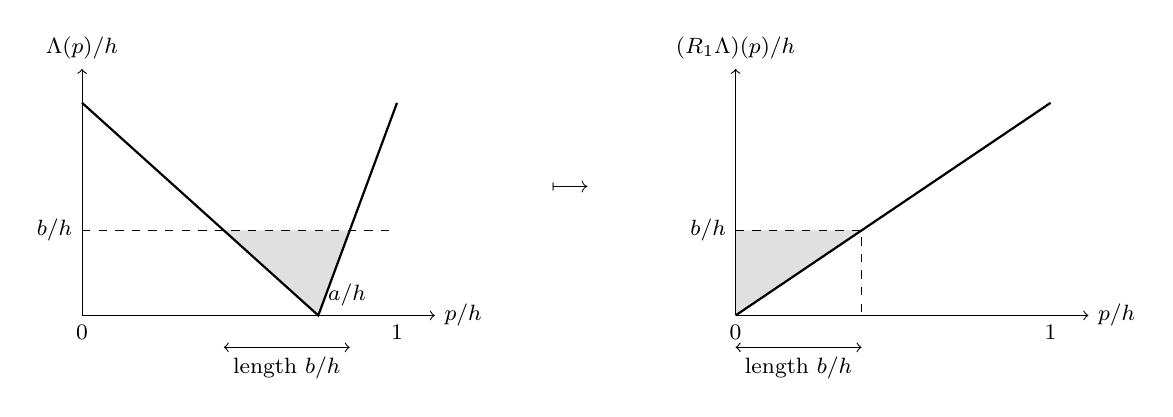
\begin{tikzpicture}[x=4cm,y=2.7cm,font=\footnotesize]
 \begin{scope}
 \fill[black!12] (0.45,0.4) -- (0.75,0) -- (0.85,0.4) -- cycle;
  \draw[->] (0,0) -- (1.12,0) node[right] {$p/h$};
  \draw[->] (0,0) -- (0,1.16) node[above] {$\Lambda(p)/h$};
  \draw[thick] (0,1) -- (0.75,0) -- (1,1);
  \draw[dashed] (0,0.4) node[left] {$b/h$} -- (1,0.4);
  \draw[<->] (0.45,-0.15) -- (0.85,-0.15) node[midway,below] {length $b/h$};
  \node[below] at (0,0) {$0$};
  \node[below] at (1,0) {$1$};
  \node[above right] at (0.75,0) {$a/h$};
 \end{scope}
 \node at (1.55,0.6) {$\longmapsto$};
 \begin{scope}[xshift=8.3cm]
  \fill[black!12] (0,0) -- (0,0.4) -- (0.4,0.4) -- cycle;
  \draw[->] (0,0) -- (1.12,0) node[right] {$p/h$};
  \draw[->] (0,0) -- (0,1.16) node[above] {$(R_1\Lambda)(p)/h$};
  \draw[thick] (0,0) -- (1,1);
  \draw[dashed] (0,0.4) node[left] {$b/h$} -- (0.4,0.4) -- (0.4,0);
  \draw[<->] (0,-0.15) -- (0.4,-0.15) node[midway,below] {length $b/h$};
  \node[below] at (0,0) {$0$};
  \node[below] at (1,0) {$1$};
 \end{scope}
\end{tikzpicture}
\caption{The linear comparison: the sublevel interval of $\Lambda$ has length $b$, so its increasing rearrangement
is $p$. The drawing uses $a/h=3/4$ ($k=16$); the identity holds for every $k\ge10$.
Consequently $K-R_1(K-P)\equiv g$, before the planar realisation error is deducted.}
\label{fig:cmp-tent}
\end{figure}

\begin{proposition}[Linear comparison datum for equal balls]\label{prop:cmp-linear}
\lean{SymplecticPacking.Params.F_eq, SymplecticPacking.Params.margin_one,
SymplecticPacking.Params.K_sub_F_ge, SymplecticPacking.Qhat.K_sub_F_q_ge,
SymplecticPacking.Qhat.full_comparison, SymplecticPacking.Qhat.qhatP_spec,
SymplecticPacking.Branch2.CubicData.ofParams_valid}
\uses{lem:cmp-tent-sublevel, thm:cmp-tent-rearrangement, def:mech-datum, S-lem:fcp-AB, S-def:fcp-eq, S-thm:pll-inner}
With the notation above let $\Delta=[0,h]$, $P(p)=3(1-3p)-k(a-p)_+$, $K(p)=c_sp$ and $F=K-P$. Then
\begin{equation}\label{eq:cmp-identity}
 F(x)=-g+c_s\Lambda(x)\qquad(x\in\R).
\end{equation}
Let $e_q=\min\bigl(h/100,\ g/(128c_s)\bigr)$ (\Sref{Definition}{def:fcp-eq}) and let $(q_t)$ be the isotopy of
\Sref{Theorem}{thm:pll-inner}, whose endpoint $q=q_1$ satisfies $\Lambda(p(q(z)))\le\pi|z|^2+4e_q$ on $\bar D(h)$.
Then $(K,(q_t))$ is a comparison datum for $(\Delta,P)$ with gap $\tfrac{31}{32}g$.
\end{proposition}

\begin{proof}
By \Sref{Lemma}{lem:fcp-AB}, $c_sA=k-3s$, $c_sB=3s$ and $3sa=3-g$. For $x\le a$:
$F(x)=c_sx-3+9x+k(a-x)=(3s-k)x+ka-3$, and $-g+c_sA(a-x)=(3s-k)x+ka-(g+3sa)=(3s-k)x+ka-3$. For $x\ge a$:
$F(x)=c_sx-3+9x=3sx-3$, and $-g+c_sB(x-a)=3sx-g-3sa=3sx-3$. This proves \eqref{eq:cmp-identity}.

By \Sref{Theorem}{thm:pll-inner}, $q_0=\mathrm{id}$, every $q_t$ maps $\bar D(h)$ onto itself and is the identity on
$\{\pi|z|^2>P_{\rm supp}\}$ for a constant $P_{\rm supp}<h$ defined there, and the generator $Q_t$ vanishes there; this
is condition~\ref{it:mech-datum-collar} of Definition~\ref{def:mech-datum} for the single outer face $p=h$. For condition~\ref{it:mech-datum-cmp}, let
$w\in\bar D(h)$ and $I=p(w)$. By \eqref{eq:cmp-identity} and $4c_se_q\le g/32$,
\[
 K(I)-(K-P)\bigl(p(q(w))\bigr)=c_sI+g-c_s\Lambda\bigl(p(q(w))\bigr)\ge g-4c_se_q\ge\tfrac{31}{32}g .\qedhere
\]
\end{proof}

Thus $K-R_1F\equiv g$ exactly (Corollary~\ref{thm:cmp-tent-rearrangement}), and the planar map costs at most $g/32$.
As $t_0\to1$ the gap $g\to0$ while the packed volume $ka^2=t_0^2\to1$. The equal-capacity branch uses
$\eta_\star=1-\rho\sqrt k$, that is $t_0=(1+\rho\sqrt k)/2$ and $g=3\eta_\star/2$.

\begin{remark}[The two four-dimensional branches]\label{rem:cmp-small-k}
The linear comparison is used when the capacities are equal, $k\ge10$ and
$\eta_\star=1-\rho\sqrt k$ lies in $(0,\frac14)$, that is $\frac34<\rho\sqrt k<1$. All other four-dimensional
inputs, including $k\le9$, use the finite scalar comparator of
\Ssec{sec:scalar-cmp}.
\end{remark}

\begin{remark}[An unequal input without linear comparison function]\label{rem:cmp-linear-fails}
In the cubic model (\Ssec{sec:cub}), given capacities $\rho_i$ are realised through auxiliary capacities
$a_i>\rho_i$ and a height $h$ with $a_i<h<\frac13$ (\Sref{Lemma}{lem:cub-auxiliary}); the profile is
$P(p)=3(1-3p)-\sum_i(a_i-p)_+$ on $\Delta=[0,h]$, and by Theorem~\ref{thm:mech-packing} any continuous minorant of $P$
may replace it. For $K(p)=\kappa p$ put $F=K-P=(\kappa+9)p-3+\sum_i(a_i-p)_+$. If $(K,(q_t))$ is a comparison datum for
$(\Delta,P)$ with gap $\gamma>0$, then, evaluating condition~\ref{it:mech-datum-cmp} of Definition~\ref{def:mech-datum} at $w=0$ and at a
preimage under $q_1$ of a maximum point of $F$ (the map $q_1$ sends $\bar D(h)$ onto itself),
\begin{equation}\label{eq:cmp-minmax}
 \min_{[0,h]}F<K(0)=0,\qquad \max_{[0,h]}F<\max_{[0,h]}K .
\end{equation}
Replacing $P$ by a smaller function increases $F$, so both inequalities only become harder to satisfy, and what
follows applies to every minorant.

Consider first the limiting data $a^*$: nine capacities $8/25$ and one capacity $7/25$, so that $\sum_ia_i^2=1$, and
$h=\frac13$, where $\int_0^hP=\frac12[1-\sum_ia_i^2-(1-3h)^2]=0$. Then $F(0)=\sum_ia_i-3=\frac4{25}$, and the slopes of
$F$ on $[0,\frac7{25}]$, $[\frac7{25},\frac8{25}]$, $[\frac8{25},\frac13]$ are $\kappa-1$, $\kappa$, $\kappa+9$. If
$\kappa<0$, then $\max F\ge F(0)>0=\max K$. If $\kappa\ge1$, then $\min F=F(0)=\frac4{25}>0$. If $0\le\kappa<1$, then
$\min F=F(\frac7{25})=\frac{7\kappa-3}{25}$ and $\max F-\max K\ge\frac4{25}-\frac\kappa3$; the larger of these two
numbers is at least $\frac9{1150}$ (equality at $\kappa=\frac{21}{46}$). So for every $\kappa\in\R$ one of the
inequalities \eqref{eq:cmp-minmax} fails by at least $\frac9{1150}$.

The bound survives perturbation. Let $\eta_0=1/2000$, $|a_i-a^*_i|\le\eta_0$ and $\frac13-\eta_0\le h<\frac13$. Then
$F$ differs from its limiting value by at most $10\eta_0$ at every $p\in[0,h]$, uniformly in $\kappa$; minima over
$[0,h]\subset[0,\frac13]$ are at least the limiting minima, $F(0)$ is still among the values, and
$\max_{[0,h]}K=\kappa h\le\kappa/3$ for $\kappa\ge0$. The three cases therefore hold with every bound lowered by
$10\eta_0=\frac1{200}<\frac9{1150}$, and \eqref{eq:cmp-minmax} fails again. Such auxiliary data are forced by the
given capacities. A comparison datum forces $\int_0^hP>0$ (integrate condition~\ref{it:mech-datum-cmp} over $\bar D(h)$, using that
$q_1$ preserves area), i.e.\ $\sum_ia_i^2+(1-3h)^2<1$. With $D=1-\sum_i\rho_i^2$ and $a_i>\rho_i$ this gives
$a_i^2-\rho_i^2<D$, hence $a_i-\rho_i<D/(2\rho_i)$, and $(1-3h)^2<D$, hence $\frac13-h<\sqrt D/3$. Therefore, if
$|\rho_i-a^*_i|\le\eta_0/2$ for all $i$ (so $\rho_i>\frac14$) and $D\le9\eta_0^2$, every admissible choice of $(a,h)$
satisfies $|a_i-a^*_i|<\eta_0$ and $h>\frac13-\eta_0$, and no linear $K$ serves; for instance
$\rho_i=(1-10^{-7})a^*_i$. The scalar construction of \Sref{Proposition}{prop:scalar-cubic-data} applies to all of these inputs.
\end{remark}
